\section{Theorie}
\label{sec:Theorie}
\subsection{Absorption von \texorpdfstring{$\beta$}{beta}-Strahlung}
Die $\beta$-Strahlung ensteht durch die Umwandlung eines Neutrons in ein Proton, oder eines Protons in ein Neutron und besteht aus Elektronen beziehungsweise Positronen.
Zusätzlich entsteht noch ein Neutrino beziehungsweise Antineutrino.
Dies wird durch folgende Gleichungen beschrieben:
\begin{align*}
  p & \Rightarrow \: n \: + \: {\beta}^{+} \: + \: \nu_\text{e} \\
  n & \Rightarrow \: p \: + \: {\beta}^{-} \: + \: \overline{\nu_\text{e}}
\end{align*}
Die freiwerden Energie verteilt sich statistisch auf die entstehenden Teilchen und somit ist das Spektrum eines $\beta$-Strahlers, wie in Abbildung \ref{fig:betaspektrum}
zu sehen, ein kontinuirliches.
\begin{figure}
  \centering
  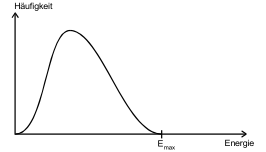
\includegraphics{pictures/betaspektrum.png}
  \caption{Emissionspektrum eines Beta-Strahlers.\cite{sample}}
  \label{fig:betaspektrum}
\end{figure}
Bei der Absoprtion von $\beta$-Strahlung am Festkörper treten eine Vielzahl von Prozessen auf.
Zum einen erleiden die Elek- und Positronen elastische Stoßprozesse. Dies führt zur Rutherfordstreuung. 
